% ch02-ml.tex -- Chapter 2: Tables, pandas and visualisation
\chapter{Tables, pandas and visualisation}\label{ch:tables}

Chapter~\ref{ch:data} taught you to treat a dataset as a bare matrix $X$:
numbers in, shapes out. Real work rarely stays in that minimal form. Columns
have names that mean something (``fare'' is not ``column 6''), rows belong to
groups you want to compare, and the fastest way to understand a table is to
plot it. This chapter upgrades the matrix to a \texttt{DataFrame} --- the same
$X$, wearing labels --- and gives you the two verbs that do $90\%$ of all
tabular work: \emph{group-and-aggregate} and \emph{reshape}. Then it does the
part most tutorials skip: how to draw a picture of the table that does not
lie to you, and how to catch the ones that do. We end on the two failure
modes that matter most --- an aggregate that hides the distribution, and an
aggregate that reverses it. Everything runs on real data: the 1912 Titanic
passenger manifest, the classic 1949--1960 airline-passenger series, and the
penguins from chapter~1.

% from-zero:begin
\begin{rulebox}[Before you start]
Chapter~1 (NumPy arrays, the dataset-as-matrix idea). \emph{Recap:} a table with named columns is a matrix with labels attached; pandas gives you those labels.
\end{rulebox}
\begin{wins}[After this chapter you can]
\begin{itemize}
\item filter, group and aggregate a table with pandas;
\item join two tables and reshape between long and wide form;
\item draw charts that do not mislead;
\item explain how an average can reverse direction when groups are merged (Simpson's paradox).
\end{itemize}
\end{wins}
\begin{principle}[How to think about this]
Exploring data is a conversation: ask a small question, look at the answer, ask the next one. Charts are arguments, so make them honest (start axes sensibly, compare like with like). Whenever a summary surprises you, split the data by a hidden group and see whether the story changes.
\end{principle}
% from-zero:end

\section{The DataFrame is a labelled matrix}\label{sec:dataframe}

A \texttt{DataFrame}\index{DataFrame} is the matrix of
chapter~\ref{ch:data} plus three things the matrix did not have: a column
name for every feature, a row label (the \emph{index}) for every sample, and
a \emph{dtype} per column that can differ between columns --- \texttt{int64}
counts, \texttt{float64} measurements, \texttt{object} strings. The matrix
inside is still an \texttt{ndarray} per column; what changed is that every
operation can be addressed by \emph{name} instead of by position.

\begin{lstlisting}[language=Python,numbers=none]
>>> df = pd.read_csv("data/titanic.csv")
>>> df.shape          # like ndarray.shape
(891, 15)
>>> df.dtypes.head(5) # one dtype per column
survived      int64
pclass        int64
sex          object
age         float64
sibsp         int64
dtype: object
>>> df["age"].mean()  # address by name, not position
29.69911764705882
\end{lstlisting}

\begin{principle}[Labels are data too]
In chapter~\ref{ch:data} the label lived \emph{outside} the matrix ($y$
beside $X$). In a DataFrame the labels live \emph{inside} the container ---
and that changes the hygiene rules, not just the syntax. A column named
\texttt{survived} is one rename away from becoming a feature by accident;
an index that silently duplicated a passenger is one groupby away from a
counting bug. Names make mistakes \emph{legible}: a wrong \texttt{df.fare}
fails loudly, a wrong \texttt{X[:,6]} fails silently.
\end{principle}

Three selection idioms cover almost everything; learn them cold.

\begin{itemize}
\item \texttt{df[df.fare > 100]} --- a boolean mask, exactly the fancy
  indexing of \S\ref{sec:loadleak}, now on named columns.
\item \texttt{df.loc[rows, cols]} --- label-based slicing:
  \par\texttt{df.loc[df.sex == "female", "age"]}
\item \texttt{df.iloc[0:5, 0:3]} --- positional slicing, identical to
  \texttt{X[0:5, 0:3]} on the underlying arrays.
\end{itemize}

\begin{checkpoint}[Reading a table's dtype story]
\texttt{titanic.csv} loads \texttt{age} as \texttt{float64} but
\texttt{pclass} as \texttt{int64}. Why the difference? (Hint: check
\texttt{df.age.isna().sum()} and \texttt{df.pclass.unique()}. What would the
dtype have been if \texttt{age} had no holes?)
\end{checkpoint}

\section{Filter, aggregate, groupby: the SQL-shaped verbs}\label{sec:groupby}

Most tabular questions decompose into four verbs, and pandas names them the
way SQL does: \emph{select} columns, \emph{filter} rows, \emph{group} by a
key, \emph{aggregate} to one number per group. The shape mental-model: a
groupby turns one $(n, d)$ table into $k$ smaller tables, and the aggregate
collapses each into one row --- an $(k, m)$ table where $m$ is how many
measures you asked for.

\begin{figure}[ht]\centering
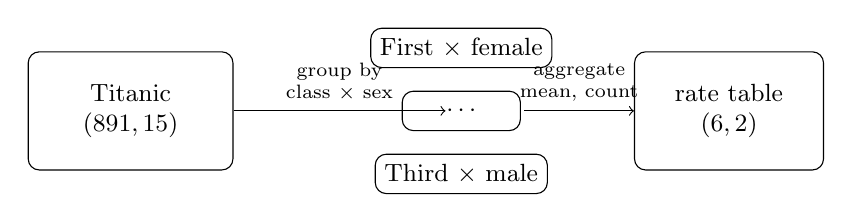
\begin{tikzpicture}[font=\small]
  \node[draw, rounded corners, minimum width=2.6cm, minimum height=1.5cm,
        align=center] (tab) at (0,0) {Titanic\\$(891, 15)$};
  \node[draw, rounded corners, minimum width=1.5cm, minimum height=0.5cm]
        (g1) at (4.2, 0.8) {First $\times$ female};
  \node[draw, rounded corners, minimum width=1.5cm, minimum height=0.5cm]
        (g2) at (4.2, 0) {$\cdots$};
  \node[draw, rounded corners, minimum width=1.5cm, minimum height=0.5cm]
        (g3) at (4.2, -0.8) {Third $\times$ male};
  \node[draw, rounded corners, minimum width=2.4cm, minimum height=1.5cm,
        align=center] (out) at (7.6,0) {rate table\\$(6, 2)$};
  \draw[->] (tab) -- node[above, font=\scriptsize, align=center]
        {group by\\class $\times$ sex} (4.0,0);
  \draw[->] (5.0,0) -- node[above, font=\scriptsize, align=center]
        {aggregate\\mean, count} (out);
\end{tikzpicture}
\caption{Split--apply--combine: \texttt{groupby} partitions the big table,
the aggregate collapses each partition to a row, and the result is a small
table indexed by the group key.}\label{fig:groupby-flow}
\end{figure}

\lstinputlisting[language=Python,caption={\texttt{code/ch02/titanic\_groupby.py}: the two idioms for one question --- \texttt{groupby+agg} produces a labelled $(6,2)$ table, \texttt{pivot\_table} the same answer laid out $(3,2)$.},label={lst:titanic}]{code/ch02/titanic_groupby.py}

Run from the repository root, it prints:

\lstinputlisting[numbers=none]{code/ch02/titanic_groupby.out.txt}

\begin{example}[WE 2.1 --- Survival by class and sex]\label{ex:titanic}
Strategy: one question, one groupby. ``Did class and sex predict survival?''
is a $(6,1)$ table away --- mean of a 0/1 column is a rate.\par
\begin{solution}
Listing~\ref{lst:titanic} answers it in three lines. The wide table is the
famous result: first-class women survived at $96.8\%$, third-class men at
$13.5\%$ --- an $83$-point gap between the luckiest and unluckiest groups.
Two cautions hidden in the same output: the \texttt{n} column matters
(third-class women, $n{=}144$, are a real estimate; a group of $n{=}5$
would be a coin flip), and ``survival by class'' is a correlation ---
the manifest does not tell you \emph{why} (boat position, queue order,
crew priorities). The table describes; it does not explain.
\end{solution}
\end{example}

\begin{figure}[ht]\centering
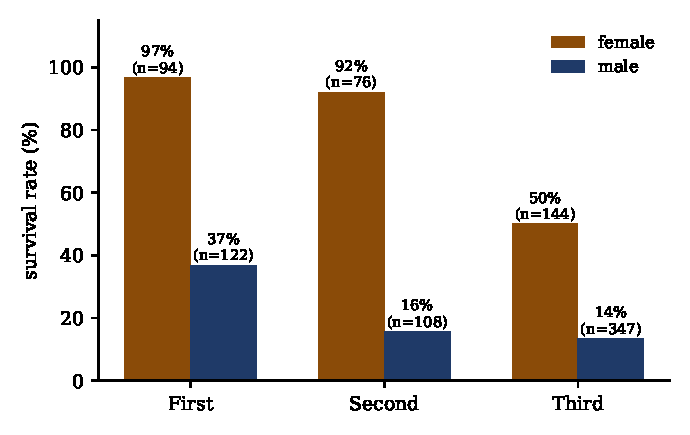
\includegraphics[width=0.72\linewidth]{figures/ch02/survival_bars.pdf}
\caption{WE 2.1 as a grouped bar chart (\texttt{figures/fig\_ch02\_survival\_bars.py}).
Counts are drawn on every bar --- $96.8\%$ of $n{=}94$ and $50.0\%$ of
$n{=}144$ are not equally trustworthy numbers.}\label{fig:survival-bars}
\end{figure}

\section{Joins and reshaping: long vs wide}\label{sec:reshape}

The same table can be stored two ways. \emph{Long} form: one row per
observation, columns are (key, variable, value) --- flexible, tidy, what
groupby wants. \emph{Wide} form: one row per entity, one column per
measurement --- readable, compact, what a table wants. The canonical tidy
rule~\cite{wickham2014}: \textbf{each variable is a column, each observation
is a row} --- keep the long form as your working truth and reshape to wide
only for presentation. The verbs:

\begin{itemize}
\item \texttt{pivot(index=..., columns=..., values=...)} --- long $\to$ wide:
  the values of one column become new column names.
\item \texttt{melt(...)} --- wide $\to$ long: column names fold back into a
  variable column.
\item \texttt{merge(other, on=key)} --- the join: match rows of two tables on
  a shared key. One line joins a grouped sum back onto the frame:
  \par\texttt{fl.merge(fl.groupby("year").passengers.sum(), on="year")}
  \par\noindent attaches each month's year total to its row --- the SQL
  \texttt{JOIN} on an aggregate, verbatim.
\end{itemize}

\begin{figure}[ht]\centering
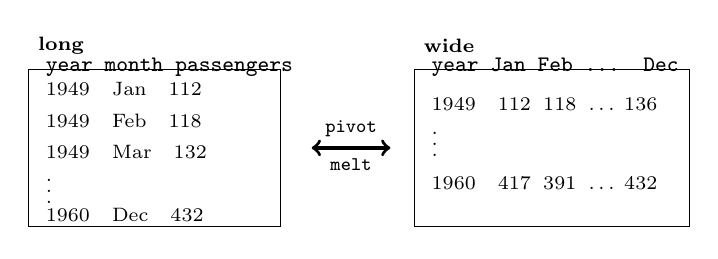
\begin{tikzpicture}[font=\scriptsize]
  % long table
  \node[anchor=west] at (0,2.3) {\textbf{long}};
  \draw (0,0) rectangle (3.2,2.0);
  \foreach \y/\a/\b/\c in {1.75/1949/Jan/112, 1.35/1949/Feb/118, 0.95/1949/Mar/132, 0.55/$\vdots$//, 0.15/1960/Dec/432}{
    \node[anchor=west] at (0.1,\y) {\a\quad\b\quad\c};}
  \node[anchor=west] at (0.1,2.02) {\footnotesize\texttt{year month passengers}};
  \draw[very thick,<->] (3.6,1) -- (4.6,1) node[midway,above]
        {\texttt{pivot}} node[midway,below] {\texttt{melt}};
  % wide table
  \node[anchor=west] at (4.9,2.3) {\textbf{wide}};
  \draw (4.9,0) rectangle (8.4,2.0);
  \node[anchor=west] at (5.0,2.02) {\footnotesize\texttt{year Jan Feb ... Dec}};
  \node[anchor=west] at (5.0,1.55) {1949\quad112\;\;118\;\;\dots\;136};
  \node[anchor=west] at (5.0,1.15) {$\vdots$};
  \node[anchor=west] at (5.0,0.55) {1960\quad417\;\;391\;\;\dots\;432};
\end{tikzpicture}
\caption{Long vs wide. Left: 144 rows of (\texttt{year}, \texttt{month},
\texttt{passengers}) --- tidy; groupby-ready. Right: the same data as a
$12\times12$ matrix --- readable; what a report wants. \texttt{pivot} and
\texttt{melt} are exact inverses: nothing is lost.}\label{fig:long-wide}
\end{figure}

\lstinputlisting[language=Python,caption={\texttt{code/ch02/pivot\_longwide.py}: long $\to$ wide $\to$ long on the real airline-passenger series; the last line proves the round trip is lossless.},label={lst:pivot}]{code/ch02/pivot_longwide.py}

\lstinputlisting[numbers=none]{code/ch02/pivot_longwide.out.txt}

\begin{example}[WE 2.2 --- One series, two shapes]\label{ex:pivot}
Strategy: know which shape each consumer wants. A grouped aggregation wants
long; a slide or a regression matrix wants wide.\par
\begin{solution}
Listing~\ref{lst:pivot} runs both directions on 144 months of real airline
data: \texttt{pivot} produces the $12\times12$ year-by-month grid (the
classic ``small multiples'' layout), \texttt{melt} folds it back, and the
set-compare at the end confirms the two forms carry identical information.
Note the months come back alphabetically (April first) --- \textbf{wide
columns sort by name, not by your intent}; if the column order matters,
reindex it. When you reach for Excel-style thinking, reach for
\texttt{pivot\_table} with an \texttt{aggfunc} instead --- it is
\texttt{pivot} that tolerates duplicate (index, column) pairs by
aggregating them.
\end{solution}
\end{example}

\section{Visualisation that does not lie}\label{sec:viz}

matplotlib\index{matplotlib} draws in two layers, and confusing them is the
root of most broken plots. The \emph{Figure} is the page; \emph{Axes} are the
panels inside it (coordinate system, ticks, spines); the \emph{artists} are
what gets inked (lines, bars, text). The idiom that keeps you sane:
\texttt{fig, ax = plt.subplots()} then call methods on \texttt{ax} ---
\texttt{ax.plot}, \texttt{ax.set\_title}, \texttt{ax.set\_ylim} --- instead
of the implicit global \texttt{plt.plot}, which guesses which axes you
meant.

\begin{figure}[ht]\centering
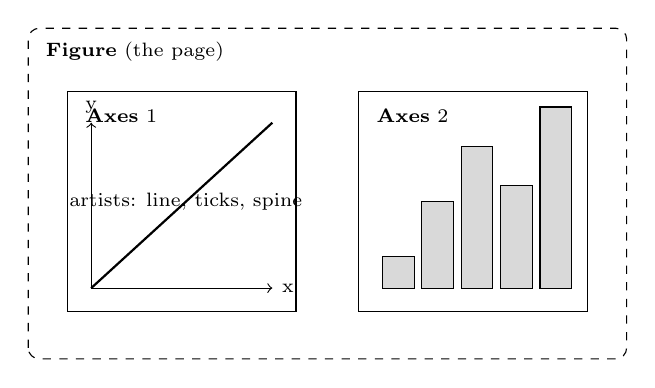
\begin{tikzpicture}[font=\scriptsize]
  \draw[rounded corners, dashed] (0,0) rectangle (7.6,4.2);
  \node[anchor=north west] at (0.1,4.15) {\textbf{Figure} (the page)};
  \draw (0.5,0.6) rectangle (3.4,3.4);
  \node[anchor=north west] at (0.6,3.3) {\textbf{Axes} 1};
  \draw[->] (0.8,0.9) -- (3.1,0.9) node[right]{x};
  \draw[->] (0.8,0.9) -- (0.8,3.0) node[above]{y};
  \draw[thick] (0.8,0.9) -- (3.1,3.0);
  \node at (2.0,2.0) {artists: line, ticks, spine};
  \draw (4.2,0.6) rectangle (7.1,3.4);
  \node[anchor=north west] at (4.3,3.3) {\textbf{Axes} 2};
  \foreach \x/\h in {4.5/0.4, 5.0/1.1, 5.5/1.8, 6.0/1.3, 6.5/2.3}{
    \draw[fill=gray!30] (\x,0.9) rectangle (\x+0.4,0.9+\h);}
\end{tikzpicture}
\caption{The matplotlib hierarchy: a Figure owns Axes; Axes own artists.
Everything you print belongs to exactly one of these --- ask ``which Axes''
before every plot call.}\label{fig:anatomy}
\end{figure}

\begin{rulebox}[Honest axes]
\begin{enumerate}
\item Bars encode length $\Rightarrow$ the $y$-axis \textbf{must include
  zero}. Truncating a bar axis is a lie of proportion; a viewer reads the
  $2\times$ visual ratio, not the $4\%$ numeric difference.
\item Lines encode position $\Rightarrow$ a non-zero axis is defensible
  \emph{if} the axis is labelled and the scale is stated. The lie is
  \emph{omission}, not the zoom.
\item Every axis gets a unit; every series gets a label or a legend; every
  figure gets a number so the text can point at it.
\end{enumerate}
\end{rulebox}

\begin{example}[WE 2.3 --- One dataset, two truths]\label{ex:honest}
Strategy: look at what the axis did, not what the line did.\par
\begin{solution}
\texttt{code/ch02/two\_plots\_one\_truth.py} plots the same airline growth
twice (Figure~\ref{fig:two-plots}). The left panel truncates the $y$-axis at
100: 1949's mean of 127 becomes a squiggle near zero and the $+276\%$ growth
reads as ``explosion''. The right panel includes zero: the same $+276\%$
reads as ``strong, steady''. Both panels are accurate. Only one is honest
\emph{in context} --- and the difference is one line of code:
\texttt{ax.set\_ylim(100, 500)} versus \texttt{ax.set\_ylim(0, 500)}. The
checklist reflex: \textbf{before reading any published chart, check where
the axis starts.}
\end{solution}
\end{example}

\begin{figure}[ht]\centering
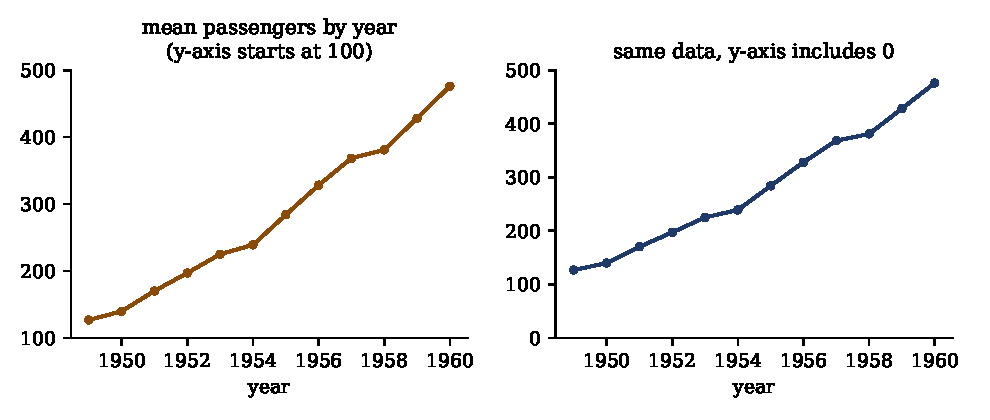
\includegraphics[width=\linewidth]{figures/ch02/two_plots.pdf}
\caption{WE 2.3 --- identical data, two axes (\texttt{code/ch02/two\_plots\_one\_truth.py}). Left: $y$ truncated at 100, growth dramatised. Right: $y$ includes 0, same growth honestly proportioned.}\label{fig:two-plots}
\end{figure}

\begin{checkpoint}[Colour vs style]
Your plot will be photocopied, printed in grey, and read by a colour-blind
reviewer. Which of these survive? (a) red vs green lines; (b) solid vs
dashed; (c) circle vs triangle markers. Design rule: encode categories in
\emph{shape or linestyle} first, colour second --- Figure~\ref{fig:scatter-matrix}
uses both (three colours \emph{and} three markers), and degrades gracefully.
\end{checkpoint}

\section{The exploration loop}\label{sec:explore}

Exploration is a loop, not a report: \emph{question $\to$ slice $\to$ plot
$\to$ new question}. The scatter matrix --- every numeric column against
every other, diagonal histograms --- is the standard first plot because it
shows $d^2$ questions at once.

\begin{figure}[ht]\centering
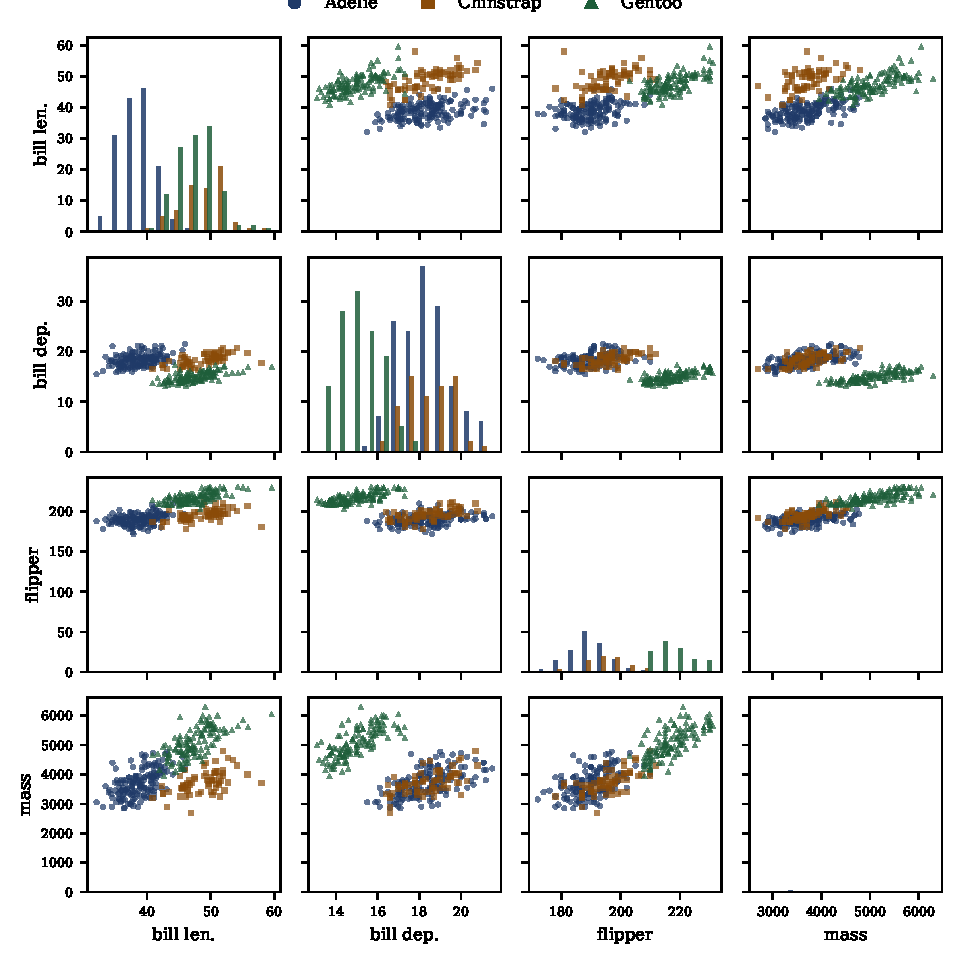
\includegraphics[width=0.86\linewidth]{figures/ch02/scatter_matrix.pdf}
\caption{Scatter matrix of the four numeric \texttt{penguins} columns
(\texttt{figures/fig\_ch02\_scatter\_matrix.py}). Gentoo separates on nearly
every pair; bill depth vs bill length slopes \emph{up} inside each species
but \emph{down} when pooled --- see \S\ref{sec:simpson}.}\label{fig:scatter-matrix}
\end{figure}

\begin{example}[WE 2.4 --- Reading the matrix]\label{ex:matrix}
Strategy: scan for three shapes --- clusters (groups you did not model),
slopes (relationships), and clouds (variance you will need).\par
\begin{solution}
Figure~\ref{fig:scatter-matrix} answers three questions in one glance.
(1)~\emph{Are the species separable?} Mostly: Gentoo's triangles sit apart
on nearly every cell --- a classifier will do well. (2)~\emph{Which features
redundate?} Bill length and flipper length slope together strongly ---
carrying both is nearly carrying one. (3)~\emph{Anything odd?} The
bill-depth vs bill-length cell (row 2, col 1) slopes \emph{down} overall yet
\emph{up} within each species --- keep that in your pocket; \S\ref{sec:simpson}
makes it the whole point. The loop continues: the separation by
\texttt{island} is the next slice, and \texttt{sex} the one after ---
exactly the mechanics of \S\ref{sec:groupby}.
\end{solution}
\end{example}

\section{When aggregation lies: Simpson's paradox}\label{sec:simpson}

Here is the failure mode that ends arguments, audits, and occasionally
careers. An aggregate that reverses \emph{every} group-level trend.

\lstinputlisting[language=Python,caption={\texttt{code/ch02/simpsons.py}: a two-department admissions table where women win \emph{both} departments and lose the pool.},label={lst:simpsons}]{code/ch02/simpsons.py}

\lstinputlisting[numbers=none]{code/ch02/simpsons.out.txt}

\begin{example}[WE 2.5 --- The pooled lie]\label{ex:simpsons}
Strategy: when a pooled rate contradicts a grouped rate, trust the grouped
rate --- the pool is a weighted sum, and the weights were rigged by who
applied where.\par
\begin{solution}
Listing~\ref{lst:simpsons} manufactures the reversal cleanly: women admit at
$85\%$ vs men's $80\%$ in History, and $24\%$ vs $20\%$ in Computer Science
--- and still lose pooled, $34.2\%$ to $68.0\%$, because $83\%$ of women
applied to the harder department. The pooled rate mixes in the application
\emph{mix}, not just the admission \emph{rates}. This is not hypothetical:
it is the structure of the 1973 Berkeley graduate-admissions
analysis~\cite{bickel1975}, and of the original 1951 paper that named the
phenomenon~\cite{simpson1951}. The rule that survives: \textbf{a pooled
statistic is a weighted average --- always ask what the weights were.}
\end{solution}
\end{example}

\begin{figure}[ht]\centering
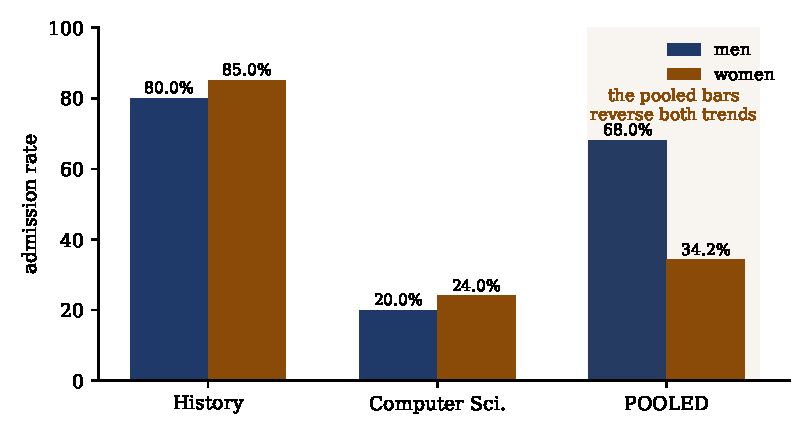
\includegraphics[width=0.72\linewidth]{figures/ch02/simpsons.pdf}
\caption{WE 2.5 --- the reversal, drawn (\texttt{figures/fig\_ch02\_simpsons.py}).
Women's bars are taller in both departments; the pooled bars flip.
Only the weights changed.}\label{fig:simpsons}
\end{figure}

And it is not just a synthetic curiosity --- your own dataset does it:

\lstinputlisting[language=Python,caption={\texttt{code/ch02/penguins\_corr\_flip.py}: pooled vs per-species correlation on \texttt{penguins} --- a real reversal on real data.},label={lst:corrflip}]{code/ch02/penguins_corr_flip.py}

\lstinputlisting[numbers=none]{code/ch02/penguins_corr_flip.out.txt}

\begin{tripwire}[Aggregates hide distributions]
A mean is one number; the data was $n$ numbers. Any pooled statistic can
reverse per-group truth --- so \textbf{plot the group breakdown before
reporting the pool}. Three reflexes: (a)~never report a rate without its
$n$; (b)~never report a pooled rate without its group rates; (c)~when a
slope looks wrong, split by the categorical column and replot ---
\texttt{penguins}' $-0.24$ pooled correlation is not evidence of
``smaller bills go with deeper bills''; it is three species with different
shapes stacked on one axis (Figure~\ref{fig:scatter-matrix}, row 2 col 1).
\end{tripwire}

\begin{wins}
\texttt{groupby + agg} for the table, \texttt{pivot} for the layout,
\texttt{merge} for the second table, and a zero-based axis for the chart.
Four verbs and one reflex carry almost every tabular question you will meet
--- and \S\ref{sec:simpson} is why the reflex is not optional.
\end{wins}

\section{Common mistakes}\label{sec:cm}

\begin{description}
\item[Aggregates hiding distributions] A mean of $4.2$ can be a tight bell
  or two spikes; a rate can be a reversal. Plot the distribution or the
  group split before trusting the number --- \S\ref{sec:simpson}.
\item[Truncated axes on bars] Bar lengths are read as ratios. If the axis
  starts at 100, a $4\%$ difference looks like $2\times$. Bars: zero or bust
  (\S\ref{sec:viz}).
\item[Pie charts] Humans compare angles badly and areas worse. Six slices
  of a pie is a bar chart that failed. If you must: label slices
  numerically, never 3-D, never more than five.
\item[\texttt{inplace=True}] \par\texttt{df.drop(col, inplace=True)}
  \par\noindent returns nothing, obscures whether a copy or a view was
  mutated, and is deprecated upstream. Assign instead:
  \par\texttt{df = df.drop(columns=col)}
\item[Chained assignment] \par\texttt{df[df.a>0]["b"]=0}
  \par\noindent may write to a temporary copy --- the
  \texttt{SettingWithCopyWarning} that is easy to silence and expensive
  to ignore. One step: \par\texttt{df.loc[df.a>0, "b"] = 0}
\item[Trusting \texttt{head()}] The first five rows are clean because
  somebody ordered them to be. Check \texttt{df.dtypes},
  \texttt{df.describe()}, and \texttt{df.isna().sum()} --- the table's
  shape of truth --- before believing any sample.
\item[\texttt{object} dtype hiding mixed types] One stray string in a
  numeric column demotes the whole column to \texttt{object}; then means
  fail \emph{two cells later}. After loading:
  \par\texttt{pd.to\_numeric(col, errors="coerce")}
  \par\noindent and count the new NaNs --- they were the strings.
\item[Aggregating before checking the index] \texttt{groupby} on a column
  with invisible whitespace (\texttt{"First"} vs \texttt{"First "}) makes
  two groups of one class. \texttt{value\_counts} the key before you trust
  the table.
\item[Forgetting the weights] A pooled average over unequal groups weights
  by $n$ silently. Sometimes that is what you want (overall rate);
  sometimes not (per-group rate). \S\ref{sec:simpson} showed the difference
  is not academic.
\end{description}

\section{Summary table}

\begin{table}[ht]\centering\small
\begin{tabularx}{\linewidth}{@{}l X l@{}}
\toprule
\textbf{Want} & \textbf{Idiom} & \textbf{Shape} \\
\midrule
subset rows & \texttt{df[df.fare>100]} / \texttt{df.loc[mask]} & $(n',d)$ \\
subset cols & \texttt{df[["age","fare"]]} / \texttt{df.iloc[:,:3]} & $(n,d')$ \\
per-group stat & \texttt{df.groupby(k).agg(mean, count)} & $(k,m)$ \\
grouped matrix & \texttt{df.pivot\_table(index, columns, values, aggfunc)} & $(r,c)$ \\
long $\to$ wide & \texttt{df.pivot(index, columns, values)} & reshape \\
wide $\to$ long & \texttt{wide.melt(...)} & reshape \\
two tables & \texttt{df.merge(other, on=key)} & $(n, d{+}d_2)$ \\
first plot & scatter matrix of numeric cols & $d^2$ panels \\
honest axis & \texttt{ax.set\_ylim(0, ...)} for bars & reflex \\
audit a pool & group first, then compare pooled vs grouped & reflex \\
\bottomrule
\end{tabularx}
\caption{Chapter 2 cheat sheet: the four verbs and the two reflexes.}\label{tab:cheat2}
\end{table}

\section*{Exercises}
\addcontentsline{toc}{section}{Exercises}

\begin{exercise}[easy]
Load \texttt{data/titanic.csv} and print \texttt{df.dtypes}. Which columns
are \texttt{float64} that ``should'' be integers, and what does that tell
you about their missing data? Verify with \texttt{isna().sum()}.
\end{exercise}
\begin{exercise}[easy]
Mean \texttt{fare} by \texttt{class} in one line. Then count rows per class
--- is the mean over $n{=}216$ First-class or $n{=}491$ Third-class
passengers more trustworthy, and why does the $n$ matter?
\end{exercise}
\begin{exercise}[easy]
Pivot \texttt{flights} to wide and pull the 1955 row. Then \texttt{melt}
the wide table back and sort --- do you recover the original rows for
1955 exactly?
\end{exercise}
\begin{exercise}[easy]
In Figure~\ref{fig:two-plots}, which single argument creates the lie?
Write the honest version for a \emph{bar} chart of the same data --- does
the rule change?
\end{exercise}
\begin{exercise}[easy]
\texttt{df.loc[0, "age"]} vs \texttt{df.iloc[0, 0]} --- what is different
about what each guarantees? When does \texttt{loc} fail that
\texttt{iloc} cannot?
\end{exercise}
\begin{exercise}[medium]
Survival by \texttt{embark\_town} $\times$ \texttt{class}: groupby the two
keys, then \texttt{unstack}. Which port's First-class rate looks anomalous
--- and what does the \texttt{n} column say about trusting it?
\end{exercise}
\begin{exercise}[medium]
Write the misleading bar chart yourself: plot survival by class with
\texttt{ylim(0.4, 0.7)}. Then fix it. Which visual feature did the
truncation distort --- bar length, spacing, or colour?
\end{exercise}
\begin{exercise}[medium]
\texttt{groupby().transform("mean")} returns a column of the
\emph{original} length, not the group count. Use it to compute each
passenger's \emph{deviation from their class mean fare}, then explain why
\texttt{agg} could not have produced that column.
\end{exercise}
\begin{exercise}[medium]
\texttt{flights}: compute each year's share of the decade's passengers with
one \texttt{merge} of a grouped sum. Then do it again with
\texttt{transform}. Which result is long-form, which is wide?
\end{exercise}
\begin{exercise}[medium]
\texttt{flights}: add a 12-month rolling mean of \texttt{passengers}
  \par\texttt{fl.passengers.rolling(12).mean()}
  \par\noindent plot it over the raw series, and say in one sentence what
  the rolling mean hides that the raw series shows.
\end{exercise}
\begin{exercise}[medium]
\texttt{penguins}: pooled \texttt{body\_mass\_g} mean vs per-species means.
Does the pooled number describe any actual penguin? Whose mean is it
closest to, and is that luck or structure?
\end{exercise}
\begin{exercise}[hard]
Construct a third department in Listing~\ref{lst:simpsons} such that women
win all \emph{three} departments and lose the pooled comparison by more
than 40 points. Verify the pooled rates numerically.
\end{exercise}
\begin{exercise}[hard]
Prove the reversal mechanically: the pooled rate for sex $s$ is
$\sum_d w_{s,d}\, r_{s,d}$ with $w_{s,d} = \mathrm{applied}_{s,d} /
\mathrm{applied}_s$. Show that flipping the weight \emph{mix} (not the
rates) is necessary and sufficient for a Simpson reversal.
\end{exercise}
\begin{exercise}[hard]
Repair the pooled comparison without pooling: standardise both sexes'
rates at a \emph{common} application mix (e.g.\ the union-average
department weights). Compute the standardised rates for
Listing~\ref{lst:simpsons} --- who ``really'' admits better?
\end{exercise}
\begin{exercise}[hard]
\texttt{penguins}: the flip of Listing~\ref{lst:corrflip} happens because
species have different bill shapes \emph{and} different prevalence. Show
numerically that reweighting the three species' counts equally changes the
pooled correlation --- find weights that flip its sign back.
\end{exercise}
\begin{exercise}[hard]
Reproduce the chained-assignment bug:
\par\texttt{df[df.fare>100]["cheap"] = 1}
\par\noindent then inspect whether \texttt{df} changed. Fix it with
\texttt{loc} in one line, and say when the warning is a false positive.
\end{exercise}

\section*{Further reading}
\addcontentsline{toc}{section}{Further reading}

\begin{itemize}
\item pandas documentation, ``10 minutes to pandas'',
  \url{https://pandas.pydata.org/docs/user_guide/10min.html}. The
  orientation lap --- indexing, selection, grouping --- run it once, keep it
  bookmarked.
\item pandas documentation, \emph{Reshaping and pivot tables},
  \url{https://pandas.pydata.org/docs/user_guide/reshaping.html}. The
  official \texttt{pivot} / \texttt{melt} / \texttt{stack} /
  \texttt{unstack} reference --- \S\ref{sec:reshape} is the first two
  floors of this page.
\item pandas documentation, \emph{Merge, join, concatenate},
  \url{https://pandas.pydata.org/docs/user_guide/merging.html}. All join
  types with honest diagrams; the one-paragraph version is our
  \texttt{merge} idiom.
\item pandas documentation, \texttt{DataFrame.groupby} reference,
  \url{https://pandas.pydata.org/docs/reference/api/pandas.DataFrame.groupby.html}.
  The full verb set --- \texttt{agg}/\texttt{transform}/\texttt{filter} ---
  worth one slow read.
\item matplotlib, ``Anatomy of a figure'',
  \url{https://matplotlib.org/stable/gallery/showcase/anatomy.html}. The
  Figure/Axes/artist map with every part labelled --- our
  Figure~\ref{fig:anatomy} with the real names.
\item matplotlib, \emph{Usage guide},
  \url{https://matplotlib.org/stable/tutorials/introductory/usage.html}.
  The official first-contact tutorial; pairs with the Schafer video below.
\item seaborn, \emph{Official tutorial},
  \url{https://seaborn.pydata.org/tutorial.html}. The next step after this
  chapter --- statistical plots on top of the same DataFrames; read the
  ``plotting functions'' section, keep the rest for later.
\item C.~O. Wilke, \emph{Fundamentals of Data Visualization}
  (free online)~\cite{wilke2019},
  \url{https://clauswilke.com/dataviz/}. The honest-visualisation book ---
  chapters 5 (directory of visualisations) and 24 (misleading axes) are this
  chapter's rules with the full theory.
\item H.~Wickham, ``Tidy data'', \emph{Journal of Statistical Software}
  59(10)~\cite{wickham2014},
  \url{https://www.jstatsoft.org/article/view/v059i10}. The long-vs-wide
  paper --- one rule (variable = column, observation = row) that organises
  every reshape decision.
\item C.~T. Bergstrom and J.~D. West, \emph{Calling Bullshit} course
  materials~\cite{callingbullshit},
  \url{https://www.callingbullshit.org/}. The citizen's guide to misleading
  charts and statistics; the ``misleading axes'' lecture is a sharper,
  longer \S\ref{sec:viz}.
\end{itemize}

\begin{rulebox}[Watch instead]
\smallskip\noindent\textbf{Best first.}
``How to spot a misleading graph'' --- TED-Ed, 4 min ---
\url{https://www.youtube.com/watch?v=E91bGT9BjYk}. Lea Gaslowitz's catalogue
of axis crimes --- the animated version of \S\ref{sec:viz} and
\S\ref{sec:cm}; watch before reading a single published chart.
\smallskip\noindent
``Python Pandas Tutorial (Part 1): Getting Started with Data Analysis'' ---
Corey Schafer, 23 min ---
\url{https://www.youtube.com/watch?v=ZyhVh-qRZPA}. Loading a CSV and the
first \texttt{DataFrame} moves --- matches \S\ref{sec:dataframe} and
\S\ref{sec:groupby}; uses Jupyter where this book uses scripts, the
pandas is identical.
\smallskip\noindent
``Matplotlib Tutorial (Part 1): Creating and Customizing Our First Plots''
--- Corey Schafer, 35 min ---
\url{https://www.youtube.com/watch?v=UO98lJQ3QGI}. The
\texttt{plt.plot} workflow of \S\ref{sec:viz} from zero; he uses the
implicit-style API --- translate each call to \texttt{ax.} methods as you
watch (the chapter's rule, not his).
Access date 2026-10-11.
\end{rulebox}

\section*{Notes}
\addcontentsline{toc}{section}{Notes}
\begin{enumerate}
\item Data sources: \texttt{titanic.csv} is the 1912 passenger manifest
  redistributed in the \texttt{seaborn-data} collection~\cite{seaborn-data}
  (891 rows, 15 columns; we read the copy in \texttt{data/});
  \texttt{flights.csv} is the Box--Jenkins airline-passenger series
  (1949--1960, 144 rows)~\cite{seaborn-data}; \texttt{penguins.csv} as in
  chapter~1~\cite{gorman2014,seaborn-data}.
\item The tidy-data rule quoted in \S\ref{sec:reshape} (variables as
  columns, observations as rows) is Wickham's formulation~\cite{wickham2014};
  it is a design guideline, not a theorem --- some algorithms want wide, some
  reports want wide, the working store stays long.
\item The Simpson's paradox example in \S\ref{sec:simpson} is synthetic but
  calibrated to the Berkeley case: the real 1973 graduate-admissions
  analysis is Bickel, Hammel and O'Connell~\cite{bickel1975}; the
  phenomenon's first formal statement is Simpson 1951~\cite{simpson1951}.
  The penguins correlation flip is measured on the real table ---
  Listing~\ref{lst:corrflip}.
\item Visualisation guidance in \S\ref{sec:viz} follows
  Wilke~\cite{wilke2019} ch.~24 and the \emph{Calling Bullshit} treatment of
  misleading axes~\cite{callingbullshit}; the bar-chart zero rule is the
  consensus rule, not universal law --- line charts and index-series are
  routinely (and fairly) zoomed.
\item Version pins for this chapter's runs: Python~3.9, pandas~2.3.3,
  matplotlib~3.9.4 --- recorded in \path{code/README.md}; all output blocks
  are verbatim captures, regenerated by the scripts.
\end{enumerate}

\section*{Hints and answers}
\addcontentsline{toc}{section}{Hints and answers}
\begin{description}
\item[2.1] \texttt{age} is \texttt{float64} because NaN is not an integer;
  \texttt{pclass} has no holes so it stays \texttt{int64}. The dtype is a
  missingness report.
\item[2.2] \texttt{df.groupby("class")["fare"].mean()} and
  \texttt{.count()}. Third class is the bigger $n$; the mean over 491
  people is the stabler estimate --- variance of a mean shrinks as $1/n$.
\item[2.3] The call
  \par\texttt{fl.pivot(index="year", columns="month", values="passengers")}
  \par\noindent gives the grid; the 1955 row should read
  January-through-December for that year. \texttt{melt} recovers the rows
  up to sort order --- months come back alphabetically, not
  chronologically.
\item[2.4] \texttt{ax.set\_ylim(100, 500)} --- one argument. For bars the
  rule is stricter: \emph{always} include zero, because bars are read as
  lengths.
\item[2.5] \texttt{loc} uses labels (row whose index is \texttt{0});
  \texttt{iloc} uses position (first row). If the index is a shuffled or
  non-integer index, \texttt{loc[0]} raises \texttt{KeyError} where
  \texttt{iloc[0]} always works.
\item[2.6] The chain
  \par\texttt{df.groupby(["embark\_town", "class"])["survived"].mean()}
  \par\noindent then \texttt{.unstack()}. Cherbourg's First-class cabin
  looks high --- check the counts before calling it a port effect; tiny
  $n$ groups swing wide.
\item[2.7] \texttt{ax.bar(...)} then
  \texttt{ax.set\_ylim(0.4, 0.7)}: the bars' \emph{lengths} now misstate
  the ratio --- spacing and colour were untouched; only the length
  encoding broke. Fix: \texttt{ylim(0, 1)} or \texttt{ylim(bottom=0)}.
\item[2.8] \texttt{transform} broadcasts each group's aggregate back to
  its rows: \texttt{df.fare} minus
  \texttt{df.groupby("class").fare.transform("mean")}. \texttt{agg}
  shrinks to one row per group; it cannot answer a per-row question.
\item[2.9] \texttt{fl.merge(...)} with
  \texttt{fl.groupby("year").passengers.sum()} on \texttt{year}, then
  divide. The merge version is long-form (one row per month still);
  \texttt{transform} gives the same long column without a join.
\item[2.10] \texttt{fl.passengers.rolling(12).mean()}, plotted over raw.
  The rolling mean hides seasonality --- the exact thing that makes the
  series interesting.
\item[2.11] Pooled $\approx 4202$~g --- no species has that mean (Adelie
  $\approx 3701$, Chinstrap $\approx 3733$, Gentoo $\approx 5076$). The pool
  describes the mixture, not any penguin; it sits nearest the middle-sized
  groups by count, not by similarity.
\item[2.12] Give the new department rates women still win (e.g.\ women
  $60\%$ vs men $50\%$) but route almost all men's applications into it ---
  pooled men rises, pooled women stays low. Check
  \texttt{pooled.rate} numerically after each edit.
\item[2.13] Decompose: pooled$_s = \sum_d w_{s,d} r_{s,d}$. Women can win
  every $r_{s,d} > r_{m,d}$ and lose when $w_{w,\cdot}$ concentrates on the
  dept where \emph{both} rates are low. The weights are the whole trick ---
  rates alone cannot reverse it.
\item[2.14] Standardised rate $= \sum_d \bar w_d\, r_{s,d}$ with common
  weights $\bar w_d$ (e.g.\ the all-applicants department shares). Compute
  it: both sexes compared on the \emph{same} mix --- women still ahead.
\item[2.15] Weight the three species' correlations by their sample shares;
  the negative pooled value comes from between-species displacement
  (Gentoo is high-length/low-depth, Adelie the reverse). Equal weights move
  the estimate toward the within-species sign.
\item[2.16] \texttt{df.loc[df.fare>100, "cheap"] = 1}. The warning is a
  false positive when the slice is provably a copy --- but you cannot see
  which it was, so \texttt{loc} is the only honest way.
\end{description}
